\section{静电势图}
前面的案例研究使用统计估计应用程序来说明选择适当级别的循环嵌套以进行并行执行、转换循环以减少内存访问干扰、
使用恒定内存来放大只读数据的内存带宽、使用 寄存器来减少内存带宽的消耗,并使用特殊的硬件功能单元来加速三角函数。 
在本案例研究中,我们使用基于常规网格数据结构的分子动力学应用程序来说明如何使用优化技术来实现全局内存访问、
合并和提高计算吞吐量。 正如我们在之前的案例研究中所做的那样,我们提出了一系列静电势图计算内核的实现,
其中每个版本都对前一个版本进行了改进。 每个版本都采用第 6 章“性能注意事项”中的一种或多种实用技术。 
前面的案例研究中使用了一些技术,但有些技术有所不同:计算结果的系统重用、线程粒度粗化和快速边界条件检查。 
该应用案例研究表明,有效使用这些实用技术可以显着提高应用程序的执行吞吐量。

\subsection{背景}
本案例研究基于视觉分子动力学 (VMD)(Humphrey 等人,1996),这是一种流行的软件系统,旨在显示、动画和分析生物分子系统。 
VMD拥有超过20万注册用户。 它是现代“计算显微镜”的重要基础,生物学家可以用它来观察微小的生命形式,
例如对于传统显微镜技术来说太小的病毒。 虽然它对分析生物分子系统有强大的内置支持,
例如计算分子系统空间网格点的静电势值(本章的重点),但它也是显示其他大型数据集的流行工具,
例如 测序数据、量子化学模拟数据和体积数据,由于其多功能性和用户可扩展性。

虽然 VMD 设计为在各种硬件上运行,包括笔记本电脑、台式机、集群和超级计算机,
但大多数用户将 VMD 用作交互式三维 (3D) 可视化和分析的桌面科学应用程序。 
对于交互使用时运行时间过长的计算,VMD 还可以以批处理模式使用来渲染电影以供以后使用。 
加速 VMD 的一个动机是使批处理模式作业足够快以供交互使用。 这可以极大地提高科学研究的生产力。 
随着 CUDA 设备在台式电脑中广泛使用,这种加速可以对 VMD 用户社区产生广泛的影响。 
迄今为止,VMD 的多个方面已通过 CUDA 得到加速,包括静电势图计算、离子放置、
分子轨道计算和显示以及蛋白质中气体迁移路径的成像。

\begin{figure}[H]
	\centering
	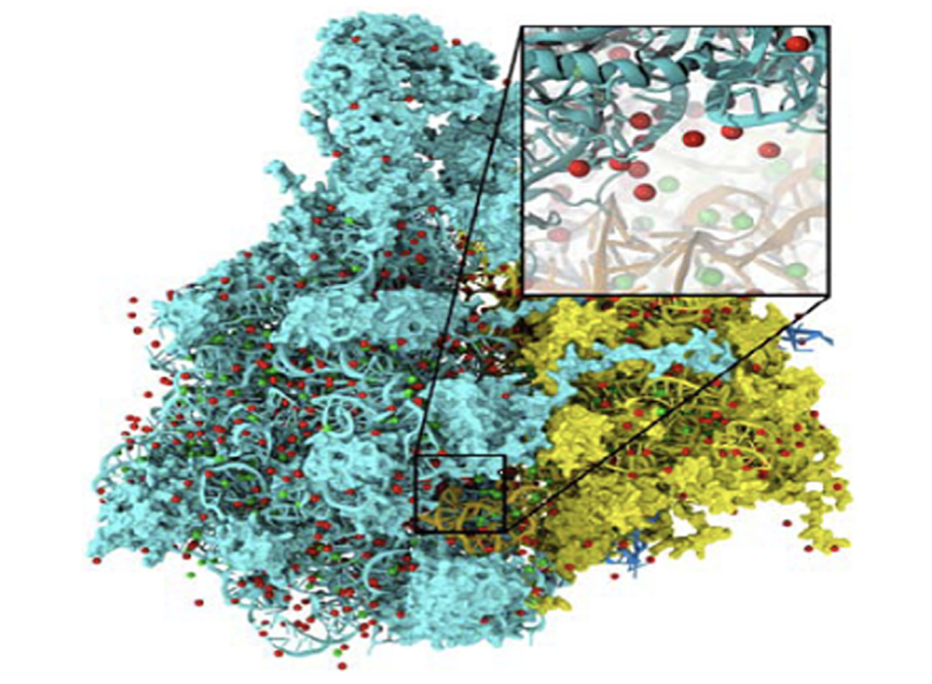
\includegraphics[width=0.9\textwidth]{figs/F18.1.png}
	\caption{\textit{用于构建分子动力学模拟稳定结构的静电势图。}}
\end{figure}

本案例研究涵盖的计算是网格空间中静电势图的计算。 此计算通常用于将离子放置到分子结构中以进行分子动力学模拟。 
图 18.1 显示了离子在蛋白质结构中的位置,为分子动力学模拟做准备。 
在此应用中,静电势图用于根据物理定律识别离子(红点)可以适应的空间位置。 
该函数还可用于计算分子动力学模拟过程中的时均电场电位图,这对于模拟过程以及模拟结果的可视化和分析很有用。

\begin{figure}[H]
	\centering
	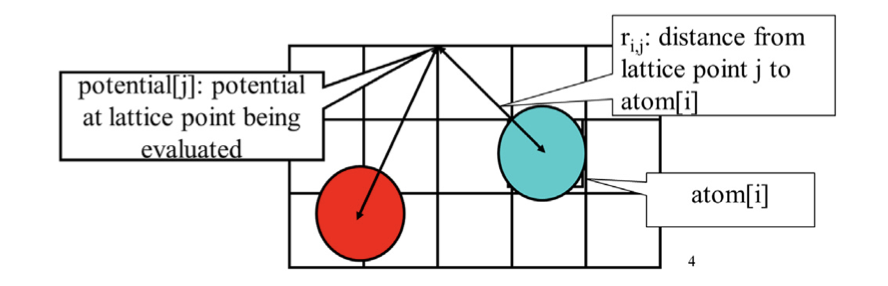
\includegraphics[width=0.9\textwidth]{figs/F18.2.png}
	\caption{\textit{atom[i]对晶格点j处的静电势(potential[j])的贡献是atom[i]。 charge/$r_{ij}$。 
	在直接库仑求和法中,晶格点j处的总电势是系统中所有原子贡献的总和。}}
\end{figure}

有多种计算静电势图的方法。 其中,直接库仑求和(DCS)是一种高精度方法,特别适合GPU(Stone et al., 2007)。 
DCS方法将每个网格点的静电势值计算为系统中所有原子的贡献之和。 
如图 18.2 所示。 原子 i 对晶格点 j 的贡献是原子 i 的电荷除以晶格点 j 到原子 i 的距离。 
由于这需要对所有网格点和所有原子进行,因此计算次数与系统中原子总数和网格点总数的乘积成正比。 
对于现实的分子系统,该乘积可能非常大。 因此,静电势图的计算传统上是作为 VMD 中的批处理作业完成的。

\subsection{核函数设计中的分散与聚集}
\begin{figure}[H]
	\centering
	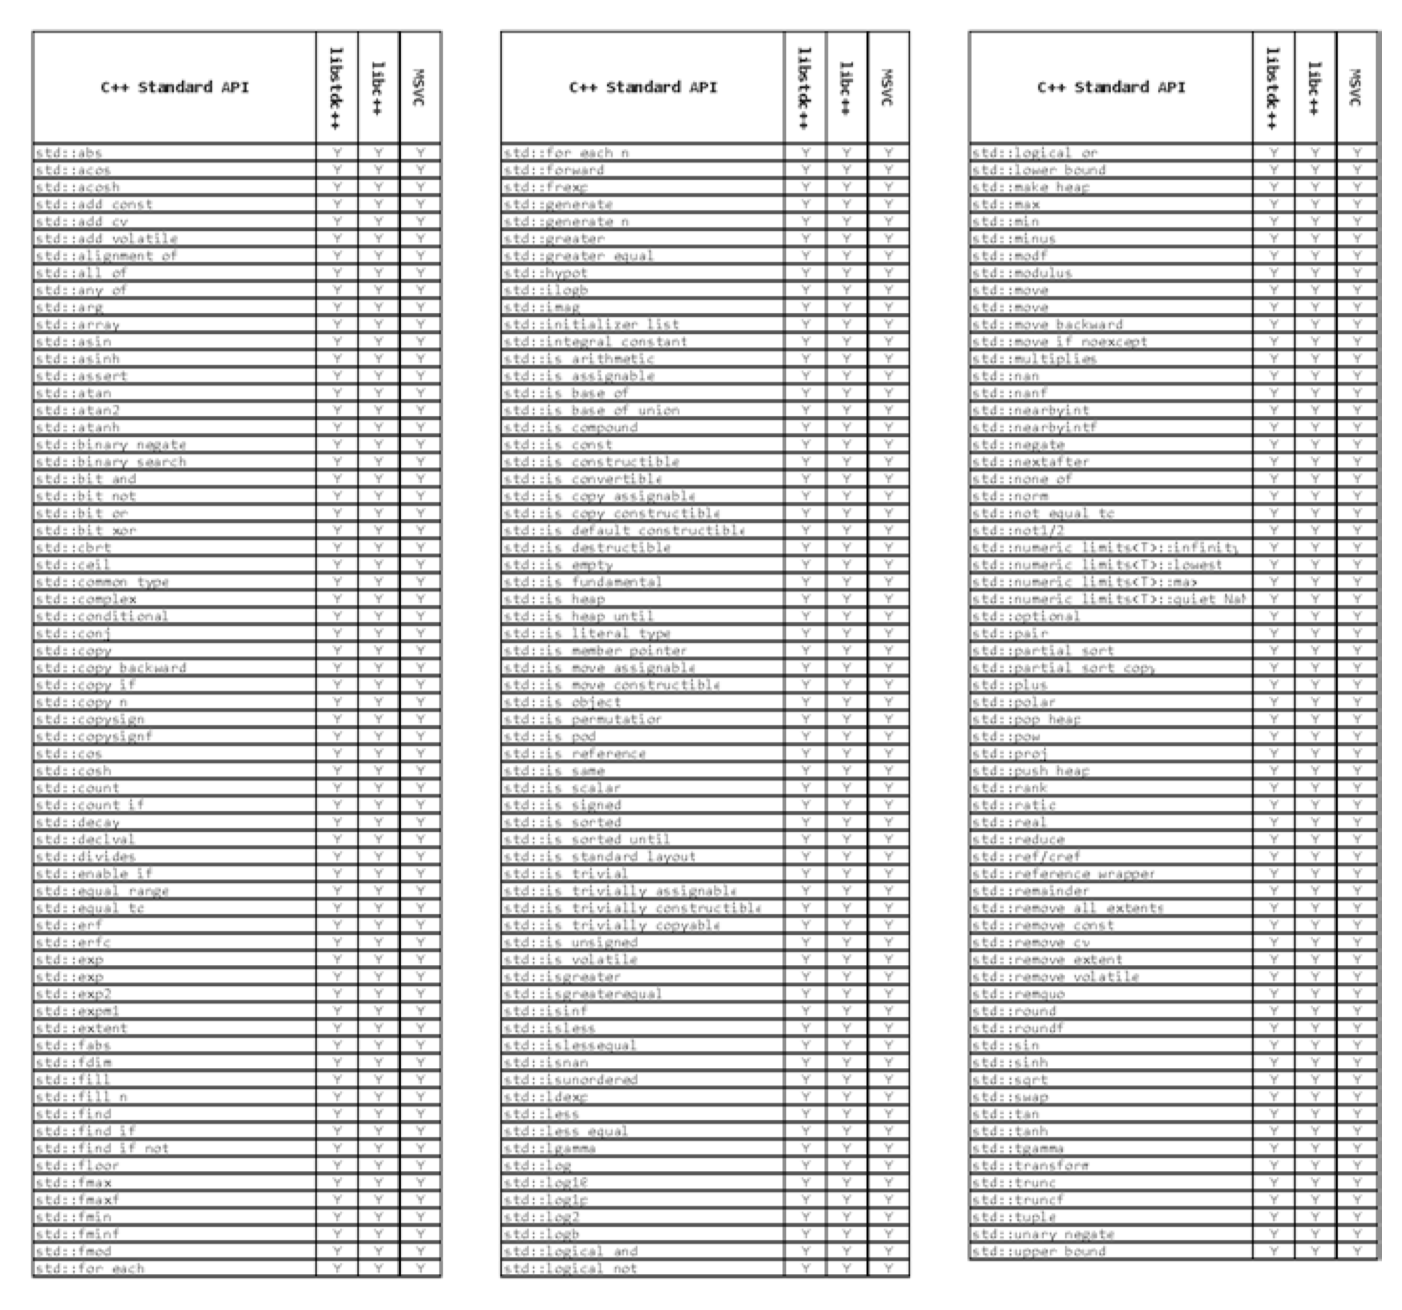
\includegraphics[width=0.9\textwidth]{figs/F18.3.png}
	\caption{\textit{二维切片的未优化直接库仑求和 C 代码。}}
\end{figure}

图 18.3 显示了 DCS 代码的基本 C 代码。 该函数被编写为处理 3D 网格的二维 (2D) 切片。 
该函数将为建模空间的所有切片重复调用。 该函数的结构非常简单,只有三层 for 循环。 
外部两个级别迭代网格点空间的 y 维度和 x 维度。 
对于每个网格点,最里面的 for 循环迭代所有原子,计算所有原子对网格点的静电势能的贡献。 
请注意,每个原子由atoms[] 数组的四个连续元素表示。 前三个元素存储原子的 x、y 和 z 坐标,第四个元素存储原子的电荷。 
在最内层循环结束时,将网格点的累加值写入网格数据结构。 然后,外部循环迭代并将执行执行到下一个网格点。

请注意,图 18.3 中的 DCS 函数通过将网格点索引值乘以网格点之间的间距来动态计算每个网格点的 x 和 y 坐标。 
这是一种均匀网格方法,其中所有网格点在所有三个维度上都以相同的距离间隔。 
该函数利用了同一切片中的所有网格点具有相同 z 坐标的事实。 该值由函数的调用者预先计算并作为函数参数 (z) 传入。 
然而,可以对图 18.3 中的顺序 C 代码进行一些优化,以显着提高其执行速度。

\begin{figure}[H]
	\centering
	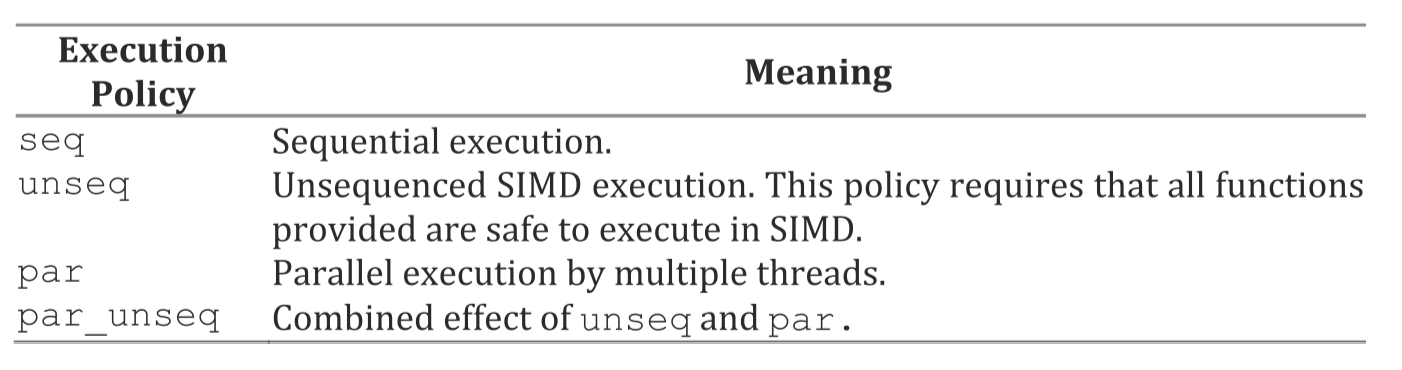
\includegraphics[width=0.9\textwidth]{figs/F18.4.png}
	\caption{\textit{用于二维切片的优化直接库仑求和 C 代码。}}
\end{figure}

图 18.4 显示了 DCS 的 C 代码,经过一些优化以提高其执行速度和效率。 
首先,图 18.3 中的最内循环(n 循环)已交换为最外循环(图 18.4 中的第 05 行)。 因此,代码会迭代所有原子。 
对于每个原子,内部循环(i 循环和 j 循环)将原子的贡献分散到所有网格点。 
正如我们在第 17 章“迭代磁共振成像重建”中讨论的,循环互换是允许的,
因为图 18.3 中的三层循环是完美嵌套的,并且所有迭代都是相互独立的。

循环交换实现了两种优化。 首先,原子与平面中所有网格点之间的距离的 z 分量是相同的,并且可以针对整个网格点切片计算一次。 
因此,计算可以在两个内部循环之外完成(第 6-7 行)。 
类似地,原子与同一行中所有网格点之间距离的 y 分量是相同的,并且可以在最内层循环之外完成(第 11-12 行)。 
相比之下,距离的 y 和 z 分量都是在图 18.3 中最里面的循环中计算的。 计算次数的大幅减少使得图 18.4 中的 C 代码速度更快。 
这些优化无法在图 18.3 中完成,因为最里面的循环会迭代所有原子,因此当原子之间的变化时,必须重新计算距离的 x、y 和 z 分量。

对于 GPU 执行,我们假设主机程序在系统内存中输入并维护原子电荷及其坐标。 它还在系统内存中维护网格点数据结构。 
DCS 内核设计用于处理静电势网格点结构的 2D 切片(不要与线程网格混淆)。 
这些网格点类似于第 8 章“模板”中讨论的离散化网格点。 对于每个 2D 切片,CPU 将其网格数据传输到设备全局内存。 
与 k 空间数据类似(第 17 章,迭代磁共振成像重建),原子信息被分成块以适合常量存储器。 
对于原子信息的每个chunk,CPU将该chunk传输到设备常量内存中,调用DCS内核计算当前chunk对当前分片的贡献,
并准备传输下一个chunk。 当前切片的所有原子信息块处理完毕后,该切片被传回以更新CPU系统内存中的网格点数据结构。 
然后系统移动到下一个切片。

\begin{figure}[H]
	\centering
	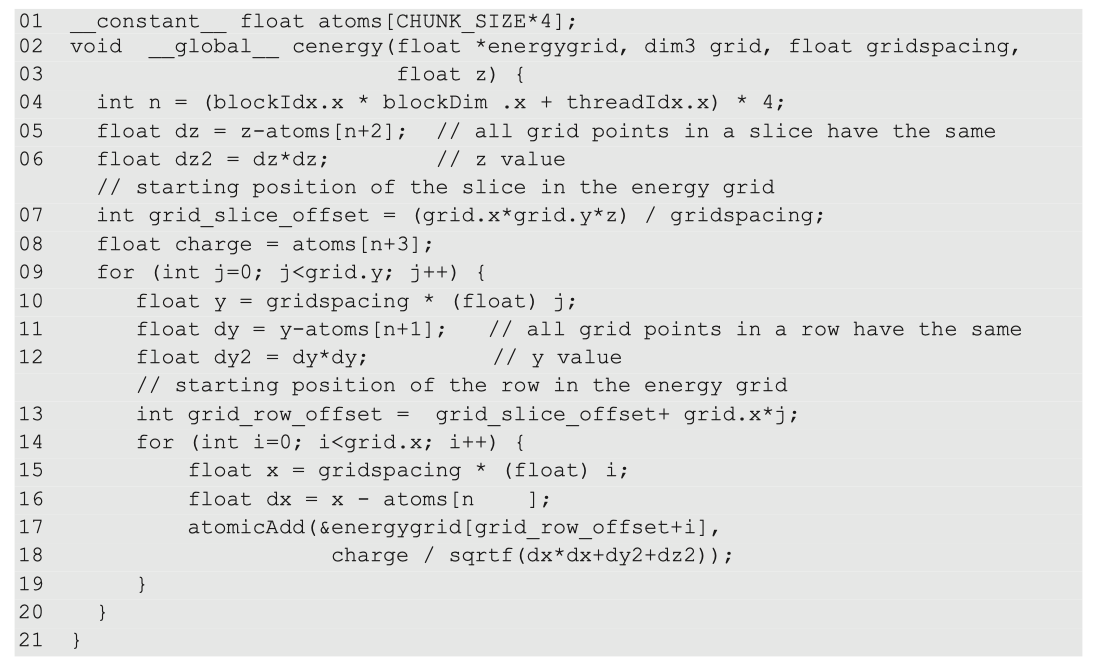
\includegraphics[width=0.9\textwidth]{figs/F18.5.png}
	\caption{\textit{使用分散方法的直接库仑求和核。}}
\end{figure}

现在让我们重点讨论DCS内核的设计。 对图 18.4 中优化的 C 代码进行并行化是很自然的。 生成的内核如图 18.5 所示。 
定义的常量 CHUNK\_SIZE 指定每次内核调用应传输到 GPU 常量内存中的原子数量。 CHUNK\_SIZE × 4 的值应小于或等于 64K。 
内核使用每个线程来实现图 18.4 中最外层循环的迭代,并将其分配的原子的贡献分散到所有网格点。 
不幸的是,正如我们在第 17 章“迭代磁共振成像重建”中了解到的那样,
这种分散的并行化方法需要原子操作来更新能量网格点(第 17-18 行),这显着降低了并行执行的速度。

正如我们在第 17 章“迭代磁共振成像重建”中了解到的,我们可以使用一种聚集方法,
其中每个线程计算所有原子对一个网格点的累积贡献。 
这是一种首选方法,因为每个线程都将写入自己的网格点,并且不需要使用原子操作。 
然而,这需要按照图18.3中未优化的C代码的顺序来排列循环; 也就是说,我们将并行化较慢的 C 实现。 
这体现了并行化应用程序中经常遇到的困境:优化的顺序代码不像未优化的顺序代码那样适合并行化。 
缺点是每个线程内的执行速度可能会大大减慢,这会降低并行化的速度优势。 我们将在本章后面回到这一点。

\begin{figure}[H]
	\centering
	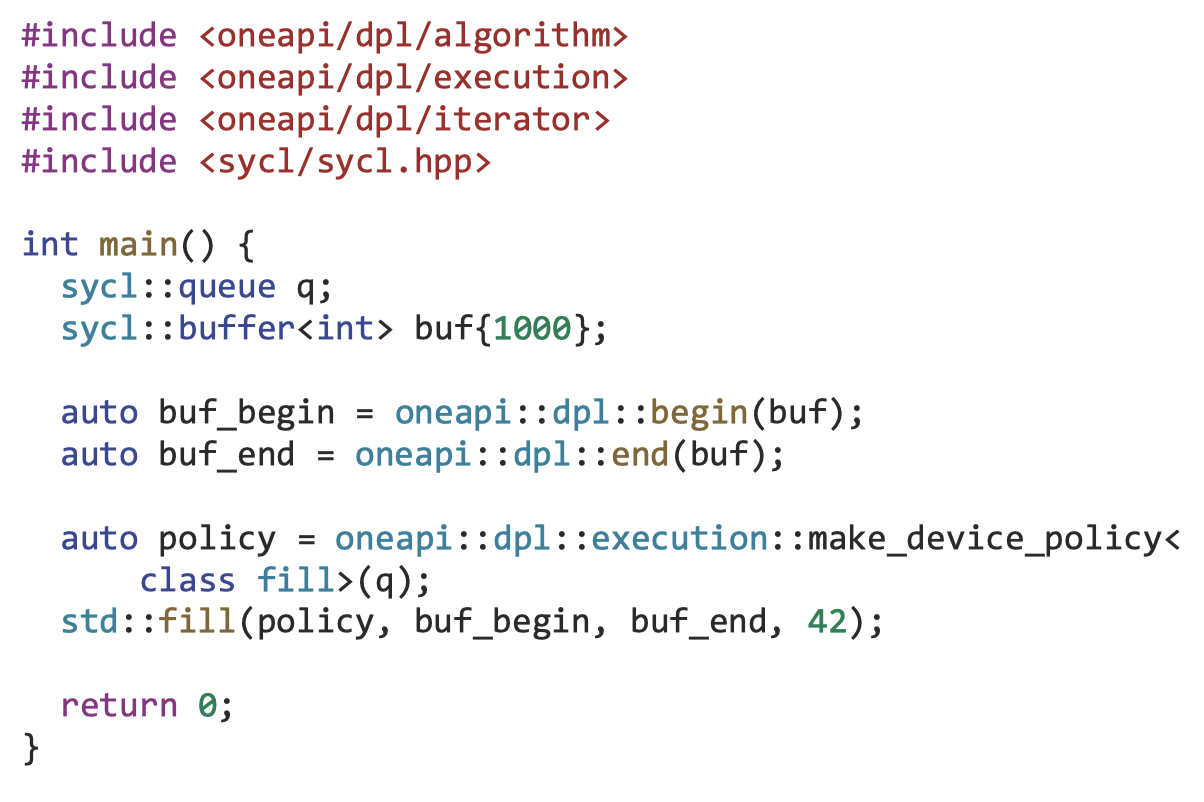
\includegraphics[width=0.9\textwidth]{figs/F18.6.png}
	\caption{\textit{使用聚集方法的直接库仑求和内核。}}
\end{figure}

图 18.6 显示了基于收集方法的内核。 内核基于图 18.3 中未优化的 C 代码。 
我们形成一个与 2D 潜在网格点组织相匹配的 2D 线程网格。 
为此,我们需要将图 18.3 的第 04-06 行中的两个外部循环修改为完美的嵌套循环,
以便我们可以使用每个线程执行两级循环的一次迭代。 
我们可以执行循环裂变(就像我们在之前的案例研究中所做的那样)或将 y 坐标(图 18.3 的第 05 行)的计算移到内部循环中。 
前者需要我们创建一个新数组来保存所有 y 值,并导致两个内核通过全局内存通信数据。 后者增加了 y 坐标的计算次数。 
在这种情况下,我们选择执行后者,因为只有少量计算可以轻松容纳在内循环中,而不会显着增加内循环的执行时间。 
吸收到内循环中的工作量比第 17 章“迭代磁共振成像重建”中的工作量小得多。 前者会增加线程执行很少工作的内核的内核启动开销。 
所选转换允许并行执行所有 i 和 j 迭代。 这是完成的计算量和实现的并行性水平之间的权衡。

在图 18.6 的内核代码内部,图 18.3 中循环的外部两级已被删除,并被内核调用中的执行配置参数取代(图 18.6 的第 04-05 行)。 
在每个线程网格内,组织线程块来计算网格结构的图块的静电电位。 在最简单的内核中,每个线程计算一个网格点的值。 
在更复杂的内核中,每个线程计算多个网格点,并利用网格点计算之间的冗余来提高执行速度。 
这是第 6 章“性能注意事项”中讨论的线程粗化优化的示例,并将在下一节中讨论。

图 18.6 中的内核的性能非常好,因为它的执行速度不受原子操作的阻碍。 
此外,快速浏览一下代码就会发现,每个线程对每访问四个内存元素执行九次浮点运算。 
每个原子的这些atoms[]数组元素被缓存在每个流式多处理器(SM)中的硬件常量高速缓存中,并且被广播到许多线程。 
跨线程大量重用这些常量内存元素使得常量缓存极其有效,消除了绝大多数 DRAM 访问。 
因此,全局内存带宽不是该内核的限制因素。

\subsection{线程粗化}
尽管图18.6中的内核通过常量缓存避免了全局内存瓶颈,但它仍然需要为每执行九个浮点运算执行四个常量内存访问指令。 
这些存储器访问指令消耗硬件资源,否则这些资源可用于增加浮点指令的执行吞吐量。 
此外,这些存储器访问指令的执行会消耗能量,这对于许多大规模并行计算系统来说是一个重要的限制因素。 
本节展示了我们可以使用线程粗化技术将多个线程融合在一起,以便 atoms[] 数据可以从常量内存中取出一次,
存储在寄存器中,并用于多个网格点。

\begin{figure}[H]
	\centering
	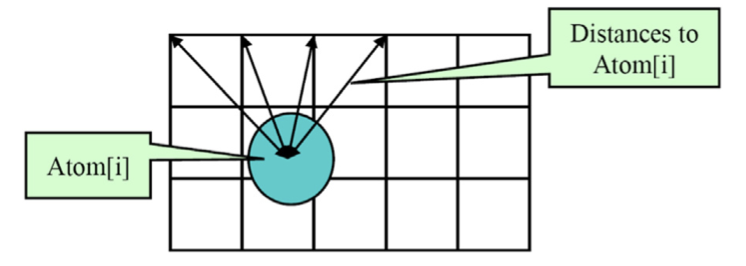
\includegraphics[width=0.9\textwidth]{figs/F18.7.png}
	\caption{\textit{在多个网格点之间重用计算结果。}}
\end{figure}

此外,如图18.7所示,同一行($y$维度)的所有能量网格点具有相同的$y$坐标。 
因此,原子的 $y$ 坐标与沿行的任何网格点的 $y$ 坐标之间的差具有相同的值。 
在图18.6的DCS内核中,在计算原子和网格点之间的距离时,这个计算是由所有线程对一行中的所有网格点冗余地完成的。 
我们可以消除这种冗余,提高执行效率。

\begin{figure}[H]
	\centering
	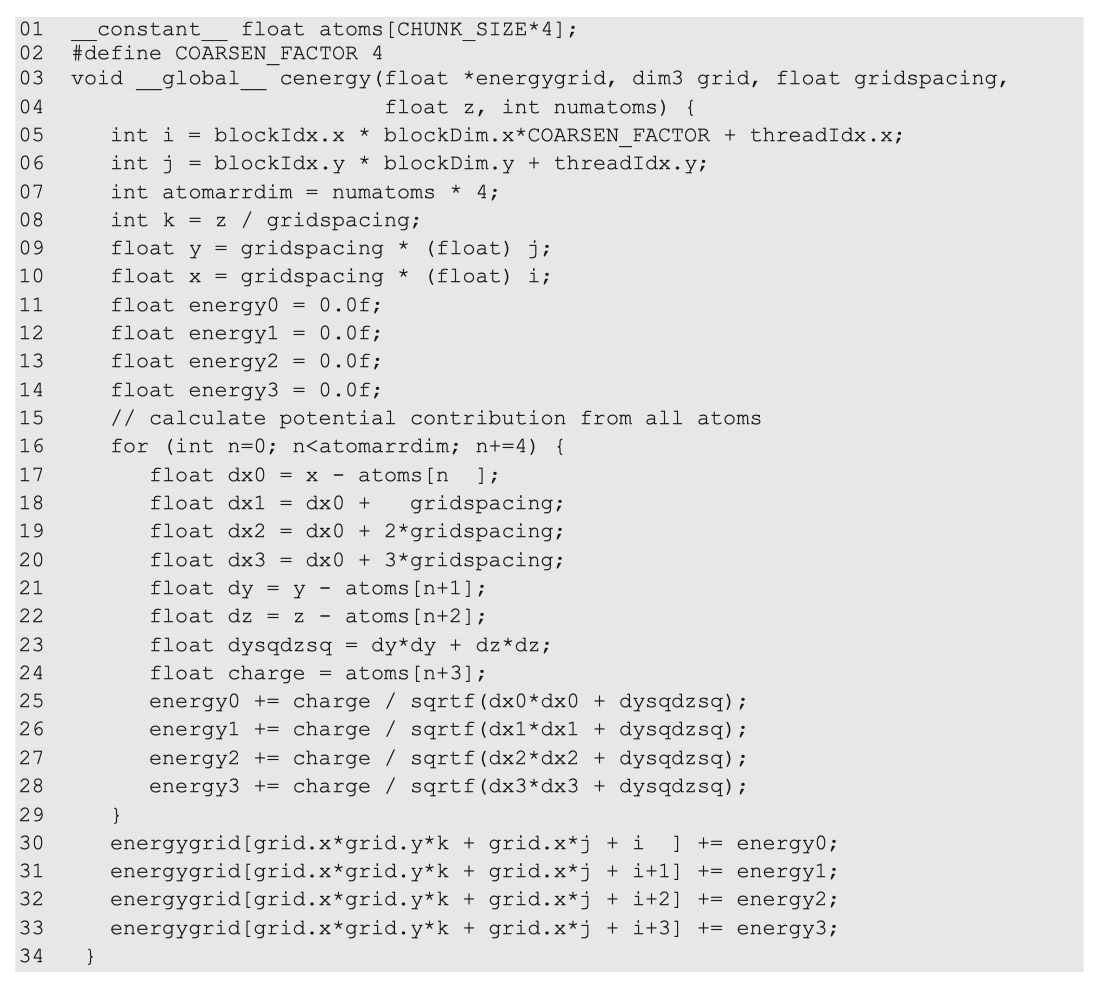
\includegraphics[width=0.9\textwidth]{figs/F18.8.png}
	\caption{\textit{带线程粗化的直接库仑求和内核。}}
\end{figure}

这个想法是让每个线程计算同一行中多个能量网格点的静电势。 图 18.8 中的内核让每个线程计算四个网格点。 
对于每个原子,代码只计算一次 dy,即 $y$ 坐标的差值(第 21 行)。 
然后,它计算表达式 $d y^{*} d y+d z^{*} d z$ 并将其保存到自动变量 Dysqdzsq 中,该变量被分配给寄存器(第 23 行)。 
该值对于所有四个网格点都是相同的。 电荷信息也可从常量存储器中获取并存储在自动可变电荷中(第 24 行)。 
因此energy0到energy3的计算都可以直接使用寄存器中存储的值。

类似地,原子的 $x$ 坐标也从常量内存中读取并用于计算 $\mathrm{dx} 0$ 到 $\mathrm{dx} 3$ (第 17-20 行)。 
总而言之,该内核消除了对其原子的 $y$ 坐标的常量内存的 3 次访问、对其原子的 $x$ 坐标的 3 次访问、
对原子电荷的 3 次访问、3 次浮点减法运算、5 次浮点运算 点乘法运算和九个浮点加法运算,用于处理四个网格点的原子。 
快速检查图 18.8 中的内核代码可以看出,
循环的每次迭代执行 4 次常量内存访问、3 次浮点减法、11 次浮点加法、6 次浮点乘法和 4 次浮点除法。 网格点。

读者还应该验证图 18.6 中的 DCS 内核版本执行了 16 次常量内存访问、12 次浮点减法、12 次浮点加法、
12 次浮点乘法和 12 次浮点除法——总共 48 次浮点除法。 对相同的四个网格点进行点操作。 
从图 18.6-图 18.6 开始 18.8 中,总共从 16 次常量内存访问和 48 次操作减少到 4 次常量内存访问和 24 次浮点操作,
减少幅度相当大。 可以预期内核的执行时间和能耗都会得到相当大的改善。

优化的代价是每个线程使用更多的寄存器。 这可能会减少每个 SM 可以容纳的线程数量。 
不过,由于寄存器的数量保持在允许的限度内,因此并不会限制GPU执行资源的占用。

\subsection{内存合并}
\begin{figure}[H]
	\centering
	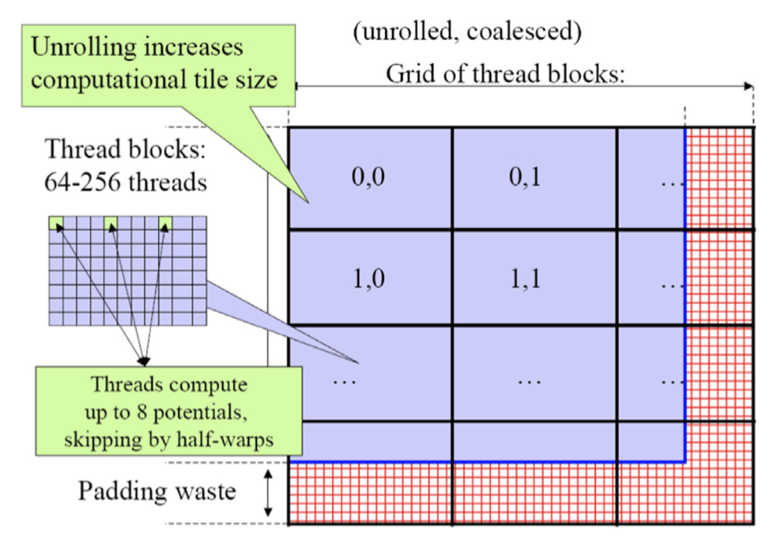
\includegraphics[width=0.9\textwidth]{figs/F18.9.png}
	\caption{\textit{组织合并写入的线程和内存布局。}}
\end{figure}

虽然图 18.8 中 DCS 内核的性能相当高,但快速分析运行表明线程执行内存写入的效率很低。 
在第 30-33 行中,每个线程写入四个相邻的网格点。 不幸的是,每个扭曲中相邻线程的写入模式将导致未合并的全局内存写入。 
有两个问题会导致内核中出现未合并的写入模式。 首先,每个线程计算四个相邻的相邻网格点。 
因此,对于写入 energygrid[] 数组的每个语句,warp 中的线程不会访问相邻位置。 
请注意,两个相邻线程访问相隔四个元素的内存位置。 
因此,一个 warp 中所有线程要写入的 32 个位置被展开,加载/写入位置之间有 3 个元素。 
这个问题可以通过将相邻的网格点分配给每个块中的相邻线程来解决。 
我们首先将 $x$ 维度中的 blockDim.x 连续网格点分配给线程。 
然后,我们将下一个 blockDim.x 连续网格点分配给相同的线程。 
我们重复分配,直到每个线程都有所需的网格点数量。 该分配如图 18.9 所示。

\begin{figure}[H]
	\centering
	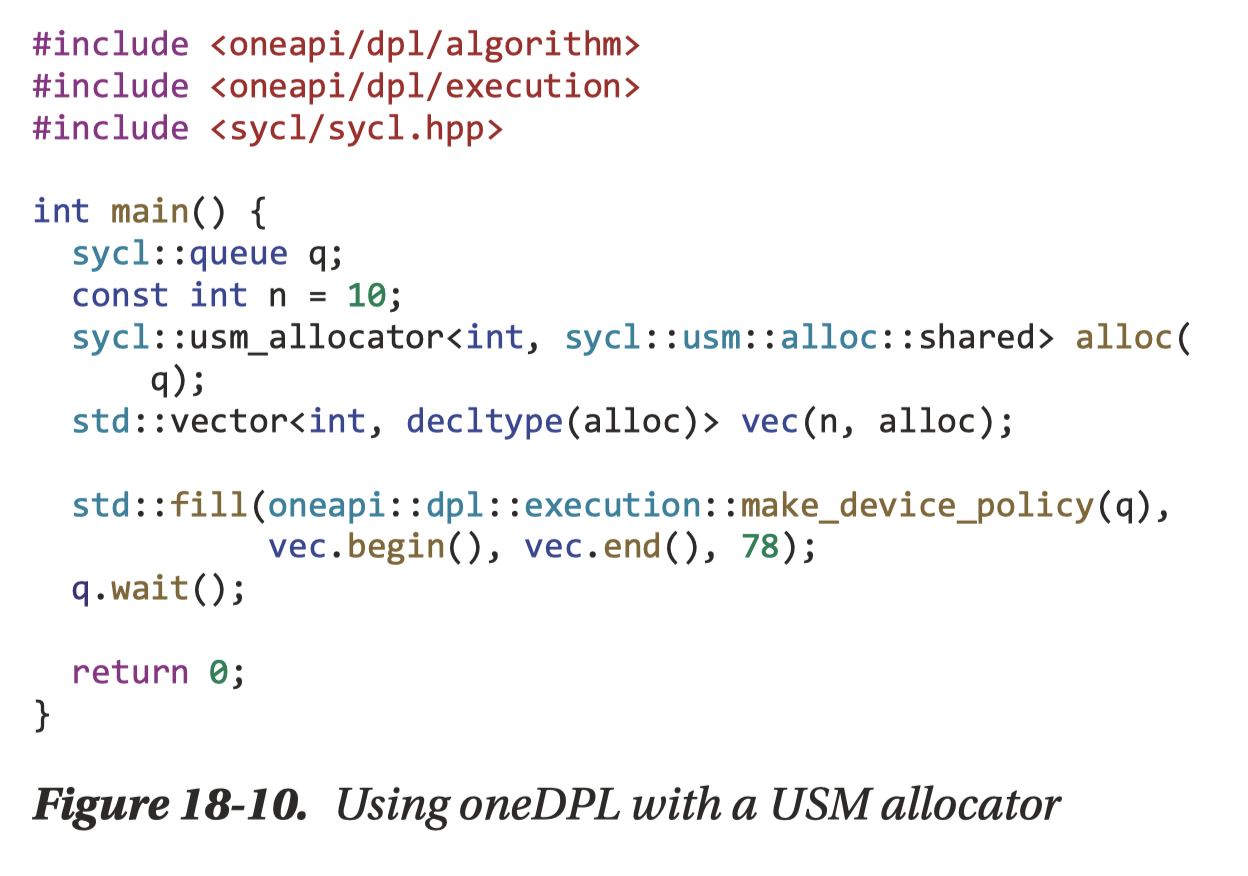
\includegraphics[width=0.9\textwidth]{figs/F18.10.png}
	\caption{\textit{具有线程粗化和内存合并的直接库仑求和内核。}}
\end{figure}

具有粗化线程粒度和合并感知的网格点分配给线程的内核代码如图 18.10 所示。 
请注意,用于计算线程分配的网格点的原子到网格点距离的 $\mathrm{x}$ 坐标偏移 blockDim.x*gridspacing。 
这反映了分配给线程的四个网格点的 $x$ 坐标彼此远离的 blockDim.x 网格点的事实。 
循环结束后,写入 energygrid 数组的内存索引也彼此远离。 
因此,对 energygrid 数组的所有写入都将被合并,并且内核的性能将比图 18.8 有所提高。

\subsection{用于数据大小可扩展性的截止分箱}
我们通常可以想出多种算法来解决给定的问题。 
有些算法比其他算法需要更少的计算步骤,有些算法比其他算法具有更高程度的并行执行,有些算法比其他算法具有更好的数值稳定性,
有些算法比其他算法消耗更少的内存带宽。 不幸的是,通常没有一种算法在所有四个方面都比其他算法更好。 
给定问题和分解策略,并行程序员通常需要选择一种算法,以实现给定硬件系统的最佳折衷方案。

一般来说,解决同一问题的替代算法应该达到相同的解决方案。 在这一要求下,可以优化计算以获得更好的效率和/或更多的并行性。 
在某些应用中,如果问题可以在最终解决方案中略有变化的情况下得到解决,那么人们通常可以想出更激进的算法策略。 
一种重要的算法策略,称为截止求和,可以通过牺牲少量的精度来显着提高静电势计算等网格算法的执行效率。 
这是基于这样的观察:许多网格计算问题都基于物理定律,
其中远离网格点的粒子或样本的数值贡献可以用隐式方法以低得多的计算复杂度来集体处理。

\begin{figure}[H]
	\centering
	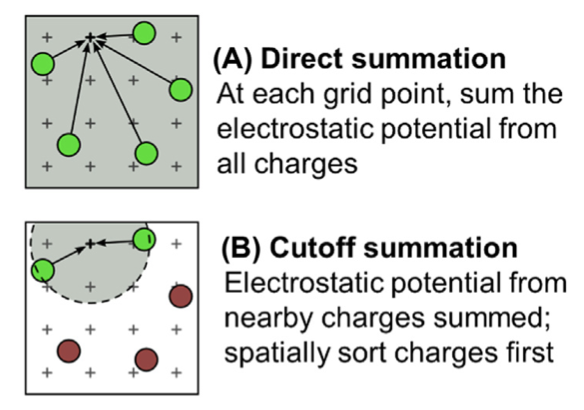
\includegraphics[width=0.9\textwidth]{figs/F18.11.png}
	\caption{\textit{(A) 截止求和与 (B) 直接求和。}}
\end{figure}

静电势计算的截止求和策略如图 18.11 所示。 图 18.11(A) 显示了本章前面部分讨论的直接求和算法。 
每个网格点接收所有原子的贡献。 虽然这是一种非常并行的方法并实现了出色的加速,但它不能很好地扩展到非常大的能源网格系统,
其中原子数量与系统体积成比例增加。 计算量随着体积的平方而增加。 
对于大容量系统,这种增加使得计算时间过长,即使对于大规模并行设备也是如此。

我们知道每个网格点都需要接收靠近它的原子的准确贡献。 远离网格点的原子对网格点处的能量值的贡献很小,因为该贡献与距离成反比。 
图 18.11(B) 用围绕网格点绘制的圆圈说明了这一观察结果。 
圆外原子(暗原子)对网格点能量的贡献很小,可以用单独的隐式方法处理。 
如果我们能够设计一种算法,其中每个网格点仅接收来自其坐标固定半径内的原子的贡献,
则该算法的计算复杂度将降低到与系统体积成线性正比。 这将使算法的计算时间与系统的体积成线性比例。 此类算法已广泛用于顺序计算。

在顺序计算中,一种简单的截止算法一次处理一个原子。 
对于每个原子,该算法迭代位于原子坐标半径内的网格点。 
这是一个简单的过程,因为网格点位于一个数组中,可以轻松地将其索引为其坐标的函数。 
截止算法的 $\mathrm{C}$ 实现可以通过对图 18.4 中 DCS 的 $\mathrm{C}$ 实现进行少量修改来导出,
方法是限制内层的 $i$ 和 $j$ 的范围。 循环到落在半径内的能量网格点。 然而,这个简单的过程并不容易移植到并行执行。 
原因就是我们在 18.2 节中讨论的:由于其分散的内存更新行为,以原子为中心的并行化效果不佳。

因此,我们需要找到一种基于网格中心分解的截止分箱算法:每个线程计算一个网格点的能量值。 
幸运的是,有一种众所周知的方法可以将直接求和算法(如图 18.10 中的算法)改编为截止分箱算法。 
罗德里格斯等人。 提出了这样一种针对静电势问题的算法(Rodrigues et al., 2008)。

该算法的关键思想是首先根据输入原子的坐标将其分类到箱中。 
每个bin对应于能量网格空间中的一个盒子,它包含坐标落入该盒子的所有原子。 
这些 bin 被实现为多维数组:$x、y$ 和 $z$ 维度以及作为 bin 中原子向量的第四维。

\begin{figure}[H]
	\centering
	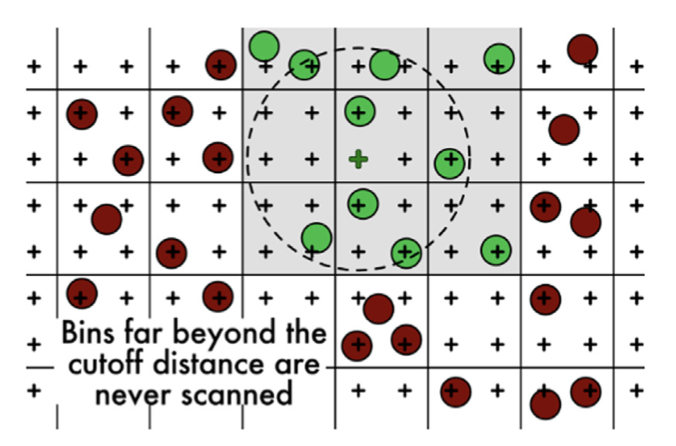
\includegraphics[width=0.9\textwidth]{figs/F18.12.png}
	\caption{\textit{网格点的邻域箱。}}
\end{figure}

我们将网格点的箱的“邻域”定义为包含可以对网格点的能量值做出贡献的所有原子的箱的集合。 
图 18.12 显示了网格点的邻域箱的示例。 请注意,网格点周围的九个箱与截止距离的圆重叠。 
为了获得正确的截止总和,我们需要确保这九个箱中的所有原子都被视为对网格点的贡献。 
请注意,邻近箱中的某些原子可能不会落入半径内。 
因此,在处理来自邻近容器之一的原子时,所有线程都需要检查该原子是否落入其半径内。 
这可能会导致扭曲中的线程之间出现一些控制分歧。

尽管图 18.12 仅显示了一层 (2D) 容器,这些容器直接围绕包含网格点作为其邻域的容器,
但实际算法通常在网格点的邻域中具有多个 3D 容器。 在这种方法中,所有线程都会迭代它们自己的邻居。 
他们使用块和线程索引来识别分配的网格点的坐标,并使用这些坐标来识别要检查的适当的箱。 
人们可以将附近的垃圾箱视为能源网格空间中的一个模板。 
然而,在给定截止半径的情况下确定邻域箱所涉及的计算可能是一个复杂的几何问题,其解决方案可能非常耗时。 
因此,邻域容器通常是为块中的所有线程定义的,并在启动网格之前准备好。

\begin{figure}[H]
	\centering
	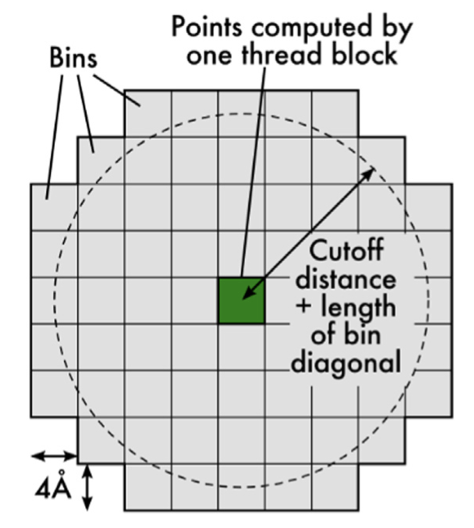
\includegraphics[width=0.9\textwidth]{figs/F18.13.png}
	\caption{\textit{识别块处理的所有网格点的邻域箱。}}
\end{figure}

图 18.13 显示了邻域 bin 的每块设计。 根据块尺寸和网格间距,可以计算出每个块所覆盖的能量网格空间的面积(3D 中的体积)。 
我们将块覆盖的区域显示为图 18.13 中的正方形。 为简单起见,我们假设每个区域也被一个垃圾箱覆盖; 
也就是说,落入同一个正方形的所有原子将被收集到同一个容器中。 
例如,如果网格间距为 $0.5 \AA$,块为 $8 \times 8 \times 8$,
则每个块将覆盖能量网格空间中的 $4 \AA \times 4 \AA \times 4 \AA$ 立方体 。 
如果我们假设分子级力计算的典型截止距离为 $12 \AA$,我们需要识别可能被 512 个圆圈中的任何一个完全或部分覆盖的所有箱,
每个圆圈都以一个网格为中心 块中线程之一覆盖的点。 
我们还可以使用保守的近似,绘制一个以 bin 中心为中心的超圆,其半径为截止距离加上 bin 对角线的一半。 
基本原理是这个超圆将覆盖以垃圾箱角为中心的所有圆。 我们可以简单地创建一个完全或部分被超圆覆盖的箱体相对位置的列表。

\begin{figure}[H]
	\centering
	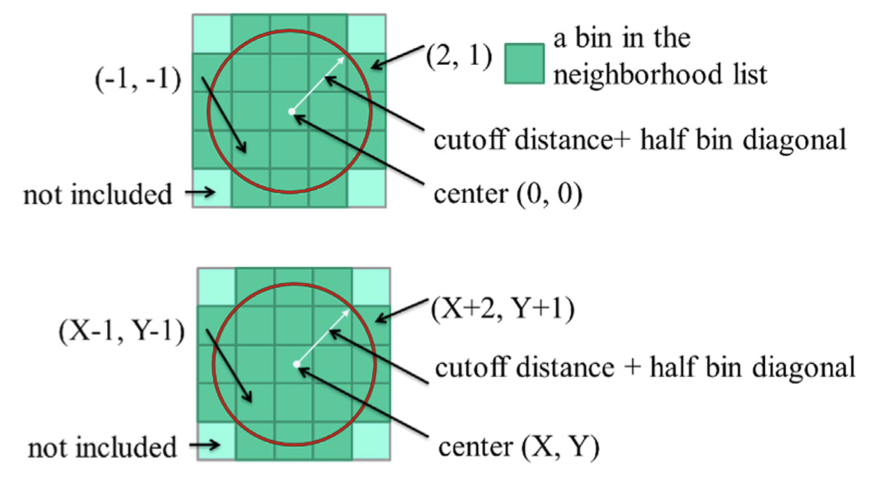
\includegraphics[width=0.9\textwidth]{figs/F18.14.png}
	\caption{\textit{使用相对偏移量的邻域列表。}}
\end{figure}

图 18.14 显示了识别邻域 bin 的一个小示例。 我们看到,对于每个 bin,有 9 个 bin 完全被超圆覆盖,12 个 bin 被部分覆盖。 
我们可以生成一个包含 $9+12=21$ 邻域箱的列表,
块中的每个线程都需要检查该列表中是否有位于该线程覆盖的网格点的截止距离内的原子。 
这些 bin 表示为 bin 坐标的相对偏移量。 
例如,被超圆完全覆盖的 9 个 bin 可以表示为列表 $(-1,-1),(0,-1)$, $(1,-1),(-1,0) 、(0,0)、(1,0)、(-1,1)、(0,1)$ 和 $(1,1)$,如图 18.14 的顶部所示。 
该列表将提供给内核,很可能作为常量内存数组。 
在内核执行期间,块中的所有线程都将迭代邻域列表。 
对于每个邻域 bin,线程将偏移量应用于块所覆盖的 bin 的坐标,并导出邻域 bin 的坐标,如图 18.14 底部所示。 
他们协作将箱中的原子加载到共享内存中,然后每个线程单独检查这些原子是否落在其分配的网格点的截止距离内。 
每个线程可以就包含或排除每个原子做出不同的决定,以贡献其分配的网格点的能量值。

截止分箱算法中计算复杂性的改进主要来自于以下事实:每个线程现在检查由大型网格系统中的邻域箱定义的小得多的原子子集。 
然而,这使得恒定记忆对于保存原子的吸引力大大降低。 
由于线程块将访问不同的邻域,因此有限大小的常量存储器不太可能容纳所有活动线程块所需的所有原子。 
这促使使用全局内存来保存更大的原子集。 为了减轻带宽消耗,块中的线程协作将每个公共邻域箱中的原子信息加载到共享内存中。 
然后所有线程检查共享内存中的原子。 分箱的一个微妙问题是分箱最终可能含有不同数量的原子。 
由于原子在网格系统中是统计分布的,所以有些箱可能有很多原子,而有些箱最终可能根本没有原子。 
为了保证内存合并,重要的是所有 bin 具有相同的大小并在适当的合并边界上对齐。 
这需要我们用电荷为 0 的虚拟原子填充许多仓,这会导致两个负面影响。 
首先,虚拟原子仍然占用全局内存和共享内存存储。 它们还消耗设备的数据传输带宽。 
其次,虚拟原子延长了其容器中真实原子很少的线程块的执行时间。

一个好的方法是将箱大小设置在一个合理的水平,该水平覆盖绝大多数箱中的原子数量,通常比箱中原子的最大可能数量小得多。 
分箱过程维护一个溢出列表。 在处理原子时,如果原子的主容器已满,则将原子添加到溢出列表中。 
设备完成内核后,生成的网格点能量值将传输回主机。 主机对溢出列表中的原子执行顺序截止算法,以完成这些溢出原子缺失的贡献。

只要溢出原子仅占原子的一小部分(例如,小于 $3 \%$ ),溢出原子的额外顺序处理时间通常比设备执行时间短。 
人们还可以设计内核,以便每次内核调用都计算网格点子体积的能量值。 
每个内核完成后,主机启动下一个内核并处理已完成内核的溢出原子。 
因此,当设备执行下一个内核时,主机将处理溢出原子。 
这种方法可以隐藏处理溢出原子时的大部分(如果不是全部)延迟,因为它是与下一个内核的执行并行完成的。

\subsection{总结}
本章介绍了在规则间隔的能量网格中并行计算静电势能的一系列决策和权衡。 
我们证明,并行化 DCS 方法的高度优化的顺序 C 实现会导致分散内核缓慢,需要大量使用原子操作。 
然后,我们展示了可以将优化程度较低的顺序 C 代码并行化为具有更高并行执行速度的聚集内核。 
我们还表明,通过线程粗化,我们可以回收优化顺序执行的大部分效率。 
我们进一步证明,通过仔细选择要折叠到每个线程中的网格点,内核可以具有完全合并的内存写入模式。

虽然 DCS 是一种计算分子系统静电势能图的高精度方法,但它不是一种可扩展的方法。 
该方法执行的操作数量与原子数量和网格点数量成比例增长。 
当我们增加要模拟的分子系统的物理体积时,我们应该预期网格点的数量和原子的数量都会与物理尺寸成比例地增加。 
因此,要执行的操作数量将近似与物理体积的平方成正比; 也就是说,要执行的操作数量将随着被模拟系统的体积呈二次方增长。 
这使得DCS方法的使用不适合模拟现实的生物系统。 
我们表明,通过稍微降低精度,使用分箱技术实现的截止求和方法可以显着提高计算的复杂性,同时保持高水平的并行性。